\documentclass[12 pt]{article} %Sets the default text size to 11pt and class to article.
%------------------------Dimensions--------------------------------------------
\topmargin=0.0in %length of margin at the top of the page (1 inch added by default)
\oddsidemargin=0.0in %length of margin on sides for odd pages
\evensidemargin=0in %length of margin on sides for even pages
\textwidth=6.5in %How wide you want your text to be
\marginparwidth=0.5in
\headheight=0pt %1in margins at top and bottom (1 inch is added to this value by default)
\headsep=0pt %Increase to increase white space in between headers and the top of the page
\textheight=9.0in %How tall the text body is allowed to be on each page
\setlength\parindent{0pt} % Removes all indentation from paragraphs

% \usepackage[T1]{fontenc}
% \usepackage{textcomp}
% \renewcommand{\familydefault}{\sfdefault}
\usepackage[latin1]{inputenc} 
\usepackage{times}
\usepackage{floatrow}
\usepackage{tgpagella}
\usepackage{lmodern}
\usepackage{fancyvrb}
\usepackage{color}
\usepackage{lipsum}
\usepackage{wrapfig}
% \usepackage[utf8]{inputenc}
\usepackage{array, xcolor}
\usepackage{graphicx}
\usepackage{fancyhdr}
\pagestyle{fancy}
\renewcommand{\headrulewidth}{0pt}
\fancyhead{}
\input{code/colorize}
\usepackage[hidelinks]{hyperref}
\usepackage{framed}
\usepackage{tikz}

\definecolor{dark-red}{rgb}{0.4,0.15,0.15}
\definecolor{dark-blue}{rgb}{0.15,0.15,0.4}
\definecolor{medium-blue}{rgb}{0,0,0.5}
\hypersetup{
    colorlinks, linkcolor={dark-red},
    citecolor={dark-blue}, urlcolor={medium-blue}
}


\begin{document}
\title{\vskip -5em \bf Near optimal A* path finding}   % type title between braces
\author{
	Andreas Valter, andva287@student.liu.se
}
\date{\today}    % type date between braces
\maketitle

\section{Introduction}
Path finding is the extraction of the shortest route between two points and is mostly a core feature that is needed to control agents in the game. 
With path finding, the user doesn't have to control all elements in the game.
Something that could be boring while playing against an AI or when there is a lot of agents that the user controls at the same time.\\

When developing computer games, each clock cycle is important. This puts a goal for each component in the game engine to be as fast as possible. 
Because when saving computation time on components, it is possible to increase the frame rate or adding more features. \\

Most computer games uses path finding to increase the game quality. For AI agents it makes it possible to go between locations.
For the user, it could make it easier to travel between places.
The most common method of choice is A* to find the shortest path between two points in a map.
The problem with using A* is that it is quite slow, depending on how the map is defined, and a lot of computation is unused in the end.\\

\section{Path finding}
\subsection{A*}
A* is basically a modified Dijkstra algorithm, that is a graph search to find the optimal path between two nodes. 
The search is done using heuristics to find probable next nodes that brings the search closer to the goal. 
For map search, the heuristics is usually the Manhattan distance from the current position to the goal position.
\begin{Verbatim}[commandchars=\\\{\}]
\PY{k}{def} \PY{n+nf}{calculateManhattanDistance}\PY{p}{(}\PY{n+nb+bp}{self}\PY{p}{,} \PY{n}{node}\PY{p}{,} \PY{n}{goal}\PY{p}{)}\PY{p}{:}
    \PY{n}{goalToNode} \PY{o}{=} \PY{n}{nodePos} \PY{o}{\PYZhy{}} \PY{n}{goal}
    \PY{k}{return} \PY{n+nb}{abs}\PY{p}{(}\PY{n}{goalToNode}\PY{o}{.}\PY{n}{x}\PY{p}{)} \PY{o}{+} \PY{n+nb}{abs}\PY{p}{(}\PY{n}{goalToNode}\PY{o}{.}\PY{n}{y}\PY{p}{)}
\end{Verbatim}

This is used to find the most likely next node, in a best-first fashion.
Figure \ref{fig:astarcat} show an example of how the algorithm works.
By adding new nodes as we traverse the map, new nodes to evaluate is added until the solution is found or until the list of nodes to evaluate is empty.
If the list of nodes is empty before a solution is found, we know that it is impossible to find a path between the start and the goal nodes.
As it show, the overhead when calculating is quite small, and this is mostly the case when using A*.
But the worst case when using it is that we are tricked to evaluate a lot of extra positions.
\begin{figure}
	\ffigbox[1.2\FBwidth]
	{\caption{A* algorithm example with a cat trying to find a bone. The values represent distance to cat, distance to bone and total sum.}}
	{\includegraphics[width=0.39\textwidth]{fig/astarcat.jpg}}
	\label{fig:astarcat}
\end{figure}
At the same time, the A* is calculated under runtime, with the possibility that the path is changed before the goal is reached.
The main benefit of using the A* algorithm is that it finds the real shortest path, in a reasonable amount of time.
This method has another flaw, if there is no path between the start and goal exist, the whole search space needs to be evaluated.
If the map is big, this gives a large cost.
But we still need to find the whole path between the nodes because that is the only way to know which way to start walking.
So a solution where we can calculate the approximate path, with high local quality would be optimal.\\

\begin{figure}	
	\ffigbox[1.2\FBwidth]
	{\caption{Map with start and goal placed. Map is divided into four clusters and nodes in black dots are added, connecting all of the clusters.}}
	{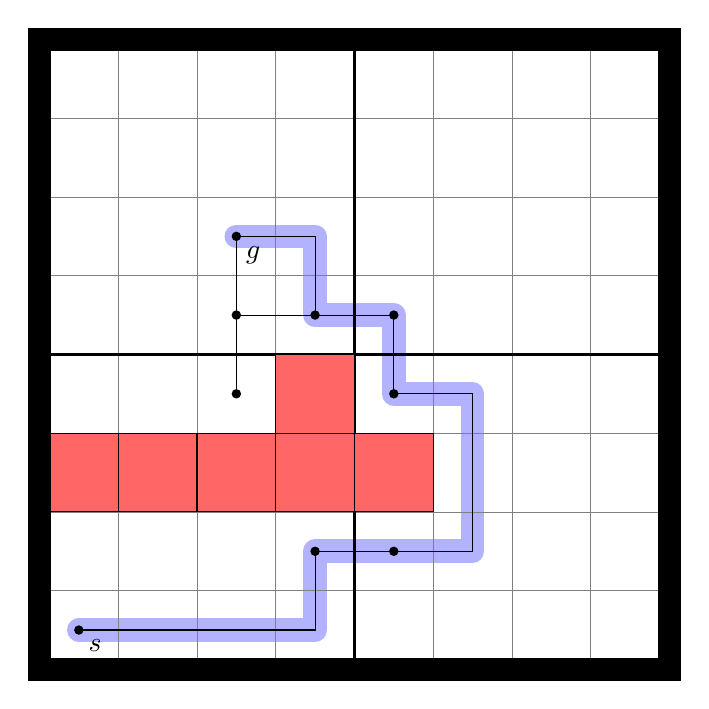
\begin{tikzpicture}
[
	bline/.style={line width=0.3cm,cap=round,join=round, color=blue!30},
	obst/.style={fill=red!60},
	myNodeLine/.style={thin,color=black!100}
]

\def\square{rectangle +(1,1)}
\def\entranceNode{circle (0.06cm)}
% Draw path
% Final path
\draw[bline] (0.5,0.5)--(3.5,0.5)--(3.5,1.5)--(5.5, 1.5)--(5.5, 3.5)--(4.5, 3.5)--(4.5, 4.5)--(3.5,4.5)--(3.5, 5.5)--(2.5,5.5);

% Draw grid 	
\draw[help lines] (0,0) grid (8,8);

% Create cluster lines
\draw[thick] (0,4)--(8,4);
\draw[thick] (4,0)--(4,8);

% Draw obstacle
\draw[obst] (2, 2) \square (3, 2) \square  (3, 3) \square  (4, 2) \square  (1, 2) \square (0, 2) \square;

% Draw border
\draw[line width=0.3cm] (0,0) rectangle +(8,8);

% Draw nodes
\draw[below right] (0.5, 0.5) node(s){$s$};
\draw[below right] (2.5, 5.5) node(t){$g$};
\fill (0.5,0.5) circle (0.06cm) (2.5,5.5) circle (0.06cm);

% Draw lines between nodes
\draw[myNodeLine](2.5, 3.5)--(2.5, 4.5) 
										(3.5, 4.5)--(4.5, 4.5) 
										(3.5, 1.5)--(4.5, 1.5);
										(4.5, 3.5)--(4.5, 4.5);

% Draw intra cluster edges
\draw[myNodeLine](4.5, 1.5)--(5.5, 1.5)--(5.5, 3.5)--(4.5, 3.5)--(4.5, 4.5)--(2.5,4.5);

% Draw connections to start and goal
\draw[myNodeLine](0.5, 0.5)--(3.5, 0.5)--(3.5, 1.5) (2.5, 5.5)--(2.5, 4.5) (2.5,5.5)--(3.5, 5.5)--(3.5, 4.5);

% Create entrance nodes
\fill (4.5,1.5) \entranceNode (3.5, 1.5) \entranceNode;
\fill (3.5, 4.5) \entranceNode (4.5, 3.5) \entranceNode;
\fill (4.5, 4.5) \entranceNode;
\fill (2.5, 4.5) \entranceNode (2.5, 3.5) \entranceNode;

\end{tikzpicture}}
	\label{fig:astarcat}
\end{figure}

\subsection{Near optimal A*}
The {\it Near optimal A*} algorithm tries to solve this problem in a clever way.
By creating a simple definition of the map beforehand, and using that representation to do fast searches, it is possible to save a lot of time.
The simple map consists of a graph structure that represents possible paths trough the map.\\

The algorithm is done in a couple of steps:\\

Firstly the map is divided into a set of clusters, with a pre specified width.
For each pair of neighbors we locate entrances, defined as points where it is possible to travel from one of the clusters to the other.
If the length of the opening between the two clusters is below a threshold, one entrance is added in the middle, if higher, two entrances are created at the edges.
All entrances are added as nodes into a graph.\\

A* is then used locally to calculate the path between all local entrances in each cluster. 
This creates a graph consisting of a lower representation of the map and possible paths between all clusters.
By temporarily adding the start and goal position to the graph, the correct path can be found by checking the path, without any need to do the costly A*.
To find the optimal path between the start and goal, we use A* again to calculate the path between them.
The difference is that we are only calculating the A* solution between two nodes in the path found in the graph.
This is more optimal because we can calculate sub steps of the path, steps that is further away is not that important so we spend time on refining the close path, knowing that we are walking in the right way.
After this, a path has been generated from the start to the goal that the agent can follow.

\section{Results}

As is shown in \autoref{fig:res1}, the application calculates a valid path that is close to the true shortest path between the start and goal nodes.
When compared to \autoref{fig:res2}, it is clear that the program uses the nodes in the search.

\begin{figure}[!h]
	\centering
	\includegraphics[width=0.5\textwidth]{fig/res2.png}
	\caption{Visualization of a randomly generated map with a calculated path draw in with points.}
	\label{fig:res2}
\end{figure}

\begin{figure}[!h]
	\centering
	\includegraphics[width=0.5\textwidth]{fig/res1.png}
	\caption{Showing the underlying structure with clusters and the generated graph that is used to calculate paths. As can be seen, the start and end nodes has been added as nodes into the graph.}
	\label{fig:res1}
\end{figure}
\clearpage
\section{Conclusion}
This implementation shows that it is possible to create changes in the A* algorithm and thereby create a faster implementation with an acceptable loss of quality.
The algorithm can quickly determine if no paths exists, only by doing searches inside the graph, making it better suited for maps that has several regions where the connection status between them is changing, like a bridge off an island that is opening for boats.
The error to the path could be reduced by a smoothing step that is applied to the final path.
It is done by removing nodes if there is a clear path to another node, without visiting a node in between.
The A* could also be applied to a node a few clusters away, depending on the cluster size.
This would make it possible to find a better path for the current vicinity, with the path trough the graph stored.
That implementation would be perfect when the goal is changing a lot because almost all the time that is spent calculating is done near the agent, where it matters.

\end{document}

